\subsection{Виртуальные машины с ОС Linux}

Для работы создан кластер из четырёх виртуальных машин с Debian~12 без графического интерфейса: один клиентский узел и три серверных. Третий сервер необходим для тома с арбитром (replica~3 arbiter~1), а также для демонстрации добавления и удаления узла из пула. Параметры узлов приведены в таблице~\ref{tab:nodes}.

\begin{table}[H]
\centering
\caption{Узлы кластера}\label{tab:nodes}
\begin{tabular}{llll}
\toprule
Имя в VirtualBox & Hostname & IP-адрес & Роль \\
\midrule
gluster-client & client & 10.0.2.10 & клиент \\
gluster-node1  & node1  & 10.0.2.11 & сервер \\
gluster-node2  & node2  & 10.0.2.12 & сервер \\
gluster-node3  & node3  & 10.0.2.13 & сервер (арбитр) \\
\bottomrule
\end{tabular}
\end{table}

Были выполнены следующие шаги.

\begin{enumerate}
  \item В VirtualBox создана NAT-сеть \code{GlusterNet} с адресным пространством \code{10.0.2.0/24} и выключенным DHCP. Для доступа к ВМ из терминала хостовой машины в сети настроен проброс портов SSH: \code{127.0.0.1:2210--2213} на порт 22 узлов \code{10.0.2.10--13}.
  \item Первая ВМ (\code{client}) установлена с нуля. В ней установлены \code{sudo} и \code{openssh-server}, задан статический IP-адрес в файле \code{/etc/network/interfaces}:
\begin{Verbatim}
auto enp0s3
iface enp0s3 inet static
    address 10.0.2.10/24
    gateway 10.0.2.1
    dns-nameservers 8.8.8.8
\end{Verbatim}
  \item В файл \code{/etc/hosts} внесены имена всех узлов:
\begin{Verbatim}
10.0.2.10 client
10.0.2.11 node1
10.0.2.12 node2
10.0.2.13 node3
\end{Verbatim}
  \item Межсетевой экран отключён (в учебных целях; в реальных проектах так делать не рекомендуется):
\begin{Verbatim}
sudo systemctl disable --now nftables
\end{Verbatim}
  \item Из выключенной ВМ \code{client} сделаны три полных клона \code{node1}, \code{node2}, \code{node3} (с новыми MAC-адресами). GlusterFS на этом этапе не устанавливался, чтобы у клонов не совпали идентификаторы узлов. На каждом клоне изменены hostname и IP-адрес, пересозданы ключи SSH-сервера и \code{machine-id}.
\end{enumerate}

Связность проверена командой \code{ping} с узла \code{client} (рисунки~\ref{fig:ping1}--\ref{fig:ping3}).

\begin{figure}[H]
  \centering
  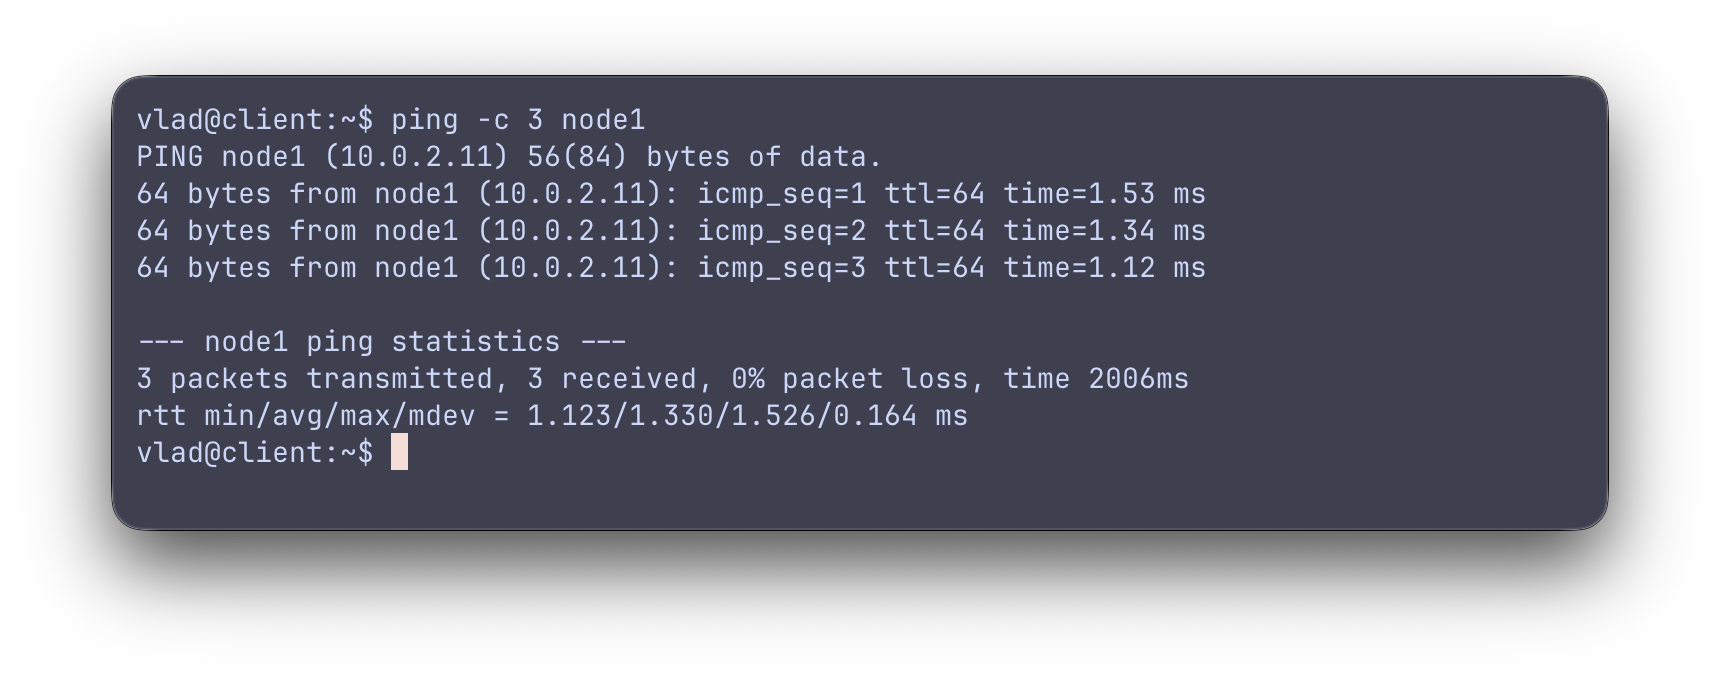
\includegraphics[max width=\linewidth,max height=0.3\textheight]{images/ping -c 3 node1.png}
  \caption{Проверка связи client\,$\to$\,node1}\label{fig:ping1}
\end{figure}
\begin{figure}[H]
  \centering
  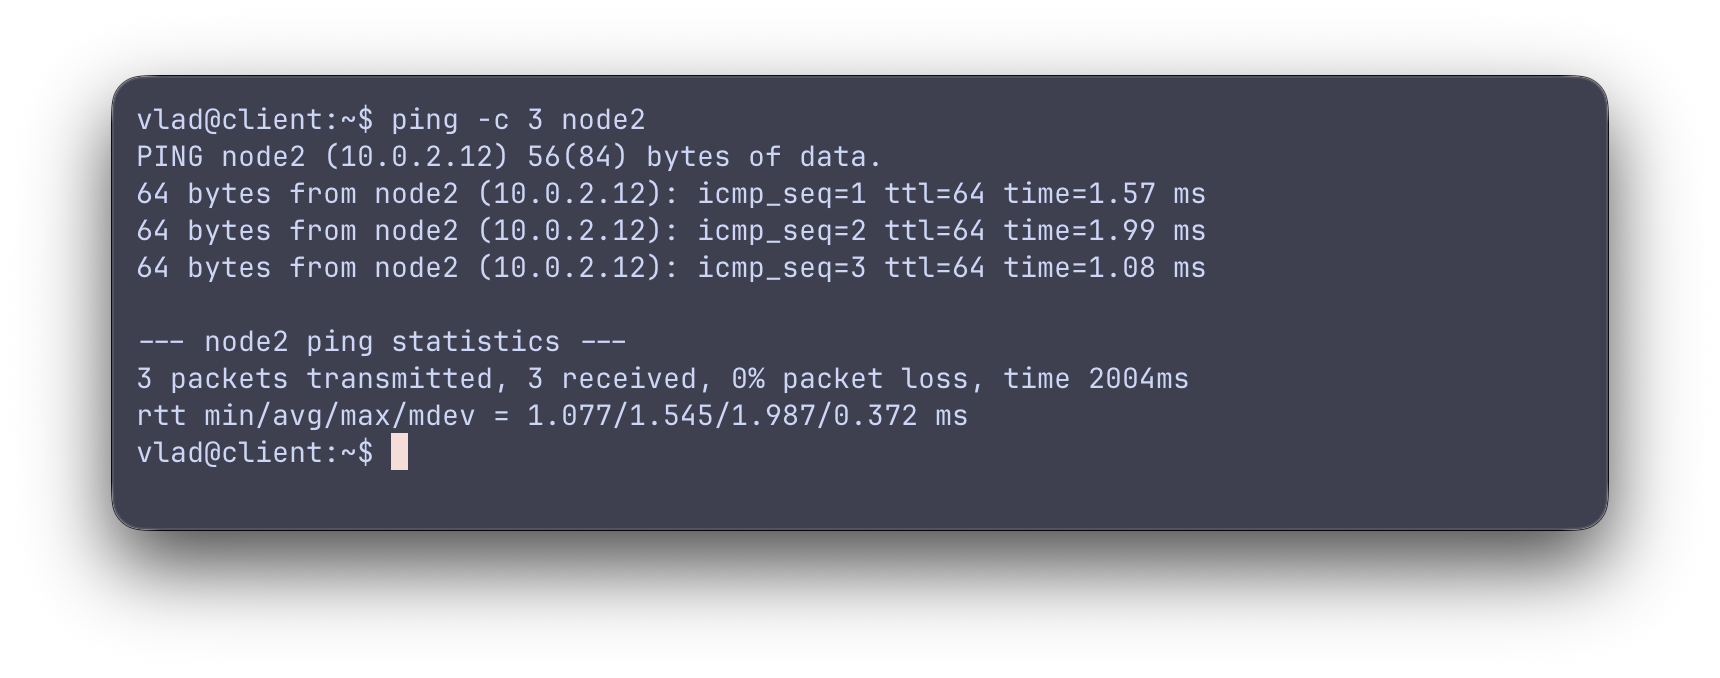
\includegraphics[max width=\linewidth,max height=0.3\textheight]{images/ping -c 3 node2.png}
  \caption{Проверка связи client\,$\to$\,node2}\label{fig:ping2}
\end{figure}
\begin{figure}[H]
  \centering
  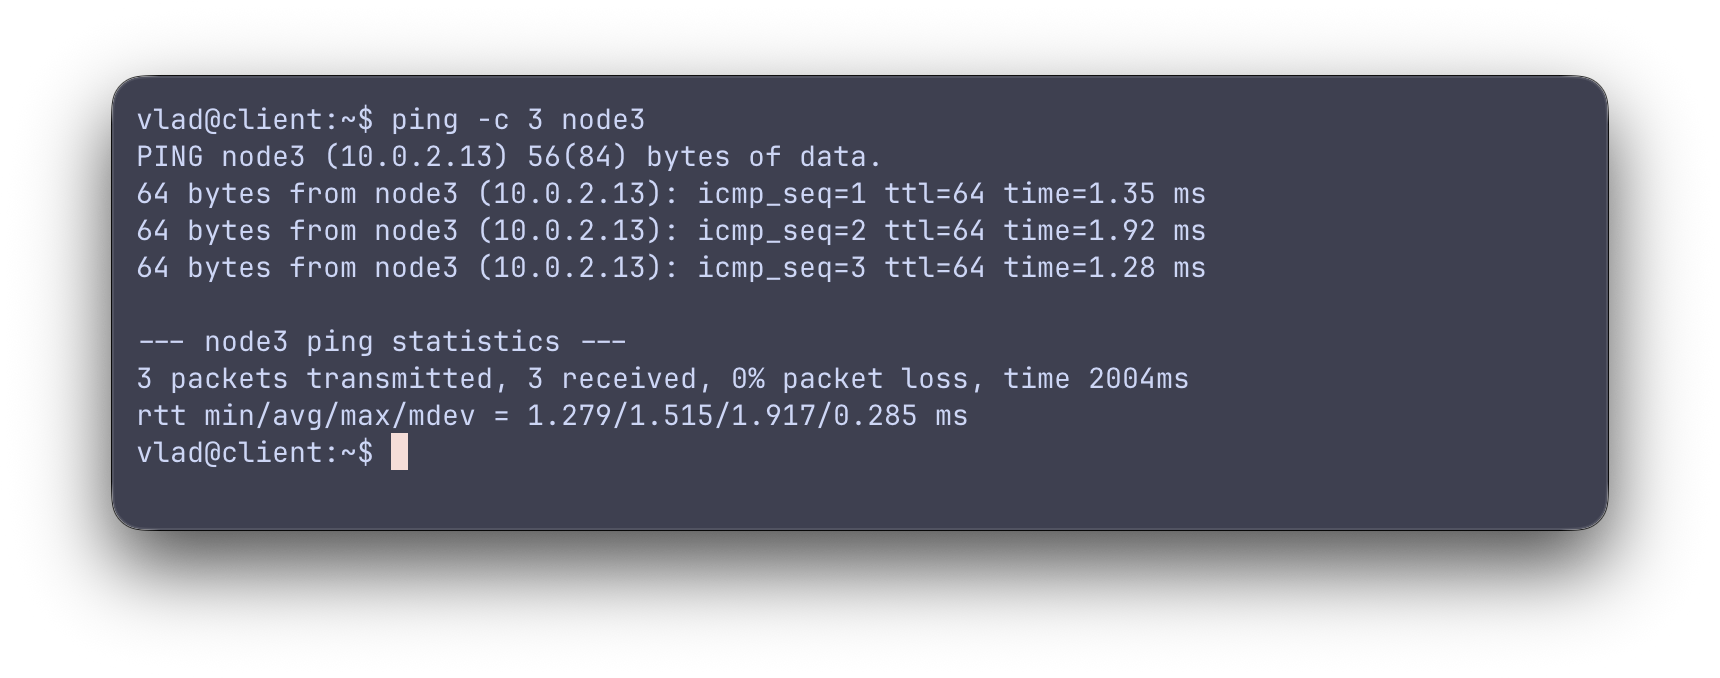
\includegraphics[max width=\linewidth,max height=0.3\textheight]{images/ping -c 3 node3.png}
  \caption{Проверка связи client\,$\to$\,node3}\label{fig:ping3}
\end{figure}
